% additional use of \usepackage{beamerthemesplit}
\documentclass{beamer}
\usepackage{beamerthemesplit} % new 
\usepackage{hyperref}
\usepackage{multimedia}
%\usepackage[spanish]{babel}
\usetheme{Montpellier}
\usecolortheme{whale}
\definecolor{verde}{rgb}{0,0,1}
\definecolor{rojo}{rgb}{1,0,0}
\definecolor{vio}{rgb}{0.5,0,0.5}
\definecolor{rosa}{rgb}{0.8,0.1,0.1}
\newcommand{\director}{Directores:\\ Mariano Dominguez \& Dante Paz}

\begin{document}
\title{A Merging Systems Detection Algorithm \& First Catalog.} 
\author{Mart\'in de los Rios, Mariano Dominguez \& Dante Paz}

\frame{\titlepage
} 

\frame{
\tableofcontents} 

\frame{
\begin{figure}[h!]
 \centering
 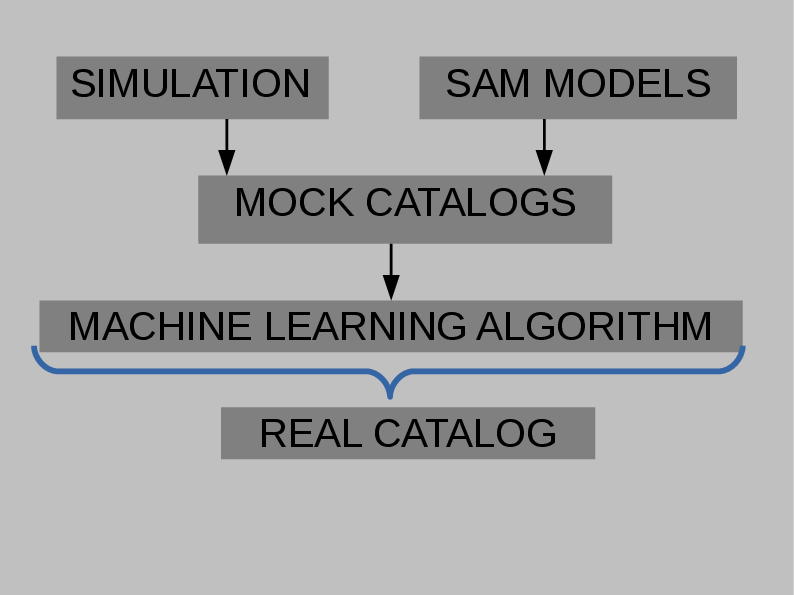
\includegraphics[scale=0.3]{./resu.png}
 % resu.pdf: 794x595 pixel, 72dpi, 28.01x20.99 cm, bb=0 0 794 595
\end{figure}

}

\section{Mock Catalog.}

\frame{
\tableofcontents[ 
    currentsection, 
    hideothersections, 
    sectionstyle=show/hide, 
    sectionstyle=show/shaded, 
    ] 
}

\subsection{Millenium}

\frame{\frametitle{Millenium Simulation}
\begin{columns}
 \begin{column}{5cm}
\begin{itemize}
 \item $N_{p}=2160^{3} $ \pause
  \item $L=500 Mpc$ \pause
 \item $m_{p}=8.61*10^{8} M_{\odot}$ \pause
 \item $\Omega_{m}=0.25$ 
 \item $\Omega_{b}=0.045$ 
 \item $\Omega_{\Lambda}=0.75$
 \item $h=0.73$ 
 \item $n_{s}=1$ 
 \item $\sigma_{8}=0.9$\pause
 \item SAM: Guo et al. 2010
 \item $Snapshots=64$
\end{itemize}
 \end{column}
 \begin{column}{5cm}
  \begin{itemize}
   \item Millenium simulation: \textit{Springel et al. 2005}.
  
  \end{itemize}

 \end{column}

\end{columns}
}

\frame{ \frametitle{Clusters identification.}
\begin{itemize}
 \item We Perform a friend-of-friend algorithm (\textit{Merchan \& Zandivares 2002 }) to the mock catalog in order to identify
the clusters. \pause
\item We assign each identified cluster with a fof-group in the simulation.
\end{itemize}



}

\frame{\frametitle{Study of the merger trees.}
\begin{itemize}
 \item Based on the subhalos merger trees, we construct the merger tree for every fof group in the simulation.
\end{itemize}

\begin{figure}[h!]
 \centering
 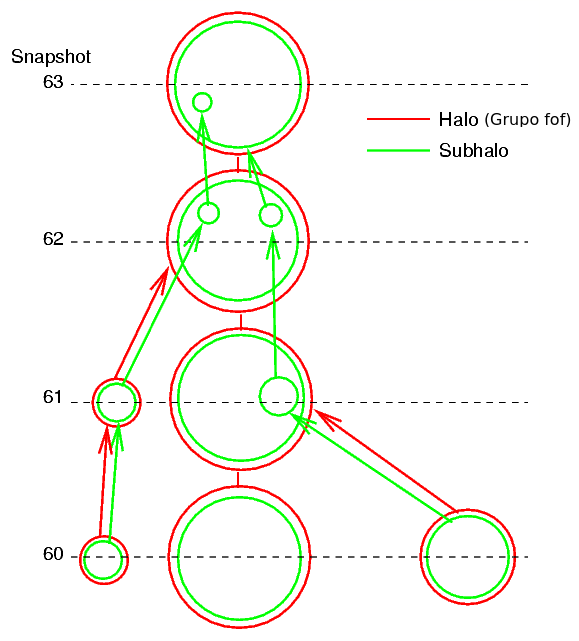
\includegraphics[scale=0.32]{./tree.png}
 % tree.eps: 0x0 pixel, 300dpi, 0.00x0.00 cm, bb=14 14 554 655
\end{figure}

}

%\frame{
%\begin{figure}[h!]
% \centering
% 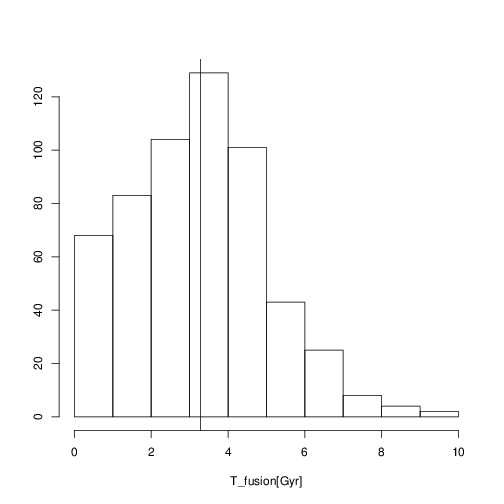
\includegraphics[scale=0.35]{./hist_tfusion.png}
 % hist_tfusion.png: 504x504 pixel, 72dpi, 17.78x17.78 cm, bb=0 0 504 504
%\end{figure}

%$\overline{T_{fusion}} \approx 3 Gyr \rightarrow $ Pinkney et al. 1996
%}

\section{Machine learning algorithm applied for identification of substructures.}
\frame{
\tableofcontents[ 
    currentsection, 
    hideothersections, 
    sectionstyle=show/hide, 
    sectionstyle=show/shaded, 
    ] 
}

\frame{
 \begin{columns}
  \begin{column}{5cm}
   \begin{itemize}
    \item Dressler-Shectman test.
    \item Non gaussianity test.
    \item Color.
    \item Number of galaxies.
   \end{itemize}
  \end{column}
  \begin{column}{5cm}
   \begin{figure}[h!]
    \centering
    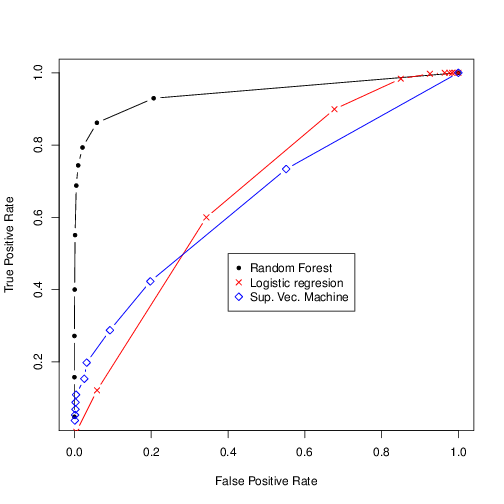
\includegraphics[scale=0.3]{./roc_curves.png}
    % roc_curves.pdf: 504x504 pixel, 72dpi, 17.78x17.78 cm, bb=0 0 504 504
   \end{figure}
  \end{column}
 \end{columns}
}

\frame{
\begin{figure}[h!]
 \centering
 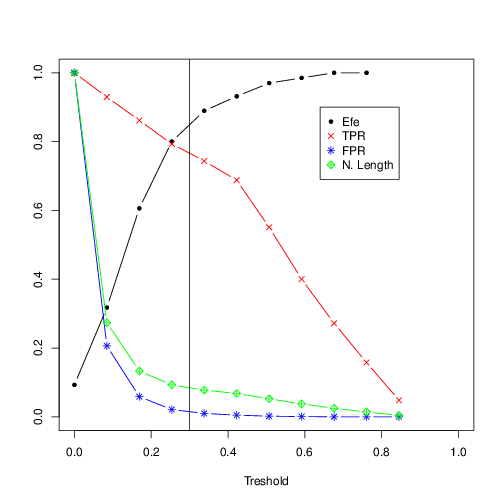
\includegraphics[scale=0.3]{./treshold.png}
 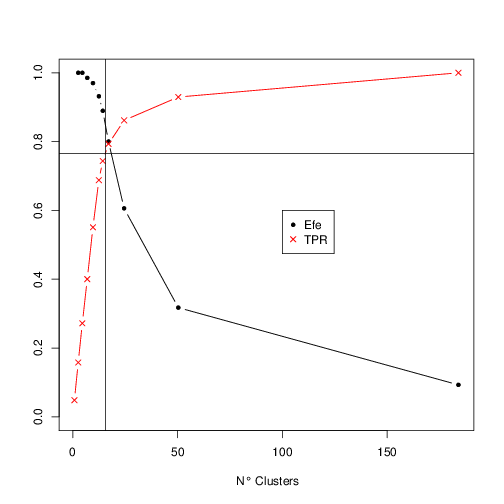
\includegraphics[scale=0.3]{./ncluster.png}
 % treshold.pdf: 504x504 pixel, 72dpi, 17.78x17.78 cm, bb=0 0 504 504
\end{figure}

}

\frame{\frametitle{Study of the identified substructures.}
\begin{tiny}
 

\begin{itemize}
\item We ran a second stage of a random forest algorithm, applied to the galaxies. \pause
\item In order to define substructures we identify clumps of galaxies based on their proximity, using a
mixture of gaussians weighted by the probability of each galaxy of being part of a substructure, calculated
with the RF. \pause

\item After the substructure identification, each one was related with the subhalo in the mock that have more galaxies in the group identified by
mclust. \pause
\item After that, we estimate the velocity dispersion and the virial radius.
 
\begin{eqnarray} \label{rvir_disp}
 R_{vir} & = & \frac{\pi}{2} \frac{ngal(ngal-1)}{\sum_{i>j}^{ngal}R_{ij}^{-1}} \nonumber\\
 \sigma &=& \frac{\sqrt{\pi}}{ngal(ngal-1)} \sum_{i=1}^{ngal-1} \omega_{i} g_{i} \nonumber\\
 \omega_{i} &=& i(ngal-i) \nonumber\\
 g_{i} &=& v_{i+1}-v_{i} \nonumber\\ 
\end{eqnarray}
\end{itemize}
\end{tiny}
}

\frame{\frametitle{Study of the identified substructures.}
%\begin{tiny}
 

\begin{itemize}
\item We compare the center of the identified substructures with the centers of the associated subhalos, finding a good estimation. \pause
\item We compare the virial radius of the identified substructures with the virial radius of the subhalos, finding that we are overestimating the real values. \pause
 \item We compare the velocity dispersion of the identified substructures with the velocity dispersion of the associated subhalos, finding that our values are
 in good concordance with the real values. 

\end{itemize}
}
%\frame{
%\begin{figure}[h!]
% \centering
% 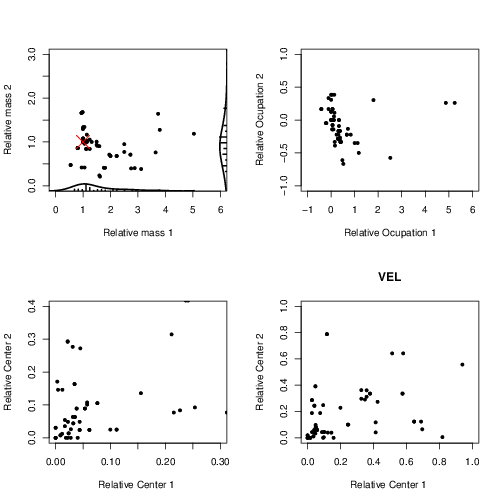
\includegraphics[scale=0.4]{./fig2.png}
 % fig2.pdf: 504x504 pixel, 72dpi, 17.78x17.78 cm, bb=0 0 504 504
%\end{figure}

%}

\frame{
\begin{tiny}
 

With this association between substructure and subhalos in the mock, we find 3 cases:

\begin{enumerate}
\item Clusters where we identify the type 0 subhalo (the principal subhalo of the fof group) and a type 1 subhalo. \pause
\item Clusters where we identify two type 1 subhalos. \pause
 \item Clusters where Mclust find two substructures that are associated to the same type 0 subhalo. \pause
\end{enumerate}
\end{tiny}

\begin{figure}[h!]
 \centering
 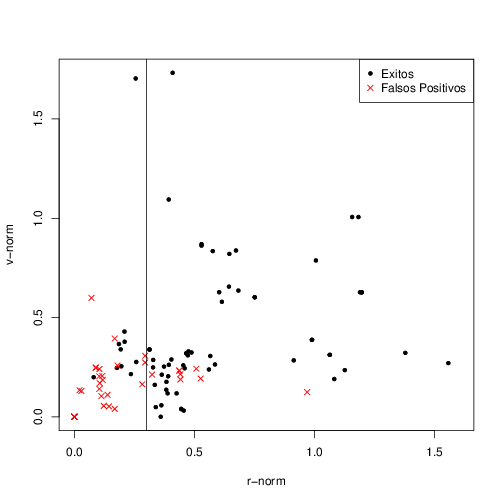
\includegraphics[scale=0.33]{./vnorm_rnorm.png}
 % vnorm_rnorm.pdf: 504x504 pixel, 72dpi, 17.78x17.78 cm, bb=0 0 504 504
\end{figure}

}


%------------------------------------------------------------------------------------------------------------------------------------------------
%------------------------------------------------------------------------------------------------------------------------------------------------
%------------------------------------------------------------------------------------------------------------------------------------------------
%------------------------------------------------------------------------------------------------------------------------------------------------
%------------------------------------------------------------------------------------------------------------------------------------------------
%------------------------------------------------------------------------------------------------------------------------------------------------
%------------------------------------------------------------------------------------------------------------------------------------------------
\section{Results.}


\frame{
\tableofcontents[ 
    currentsection, 
    hideothersections, 
    sectionstyle=show/hide, 
    sectionstyle=show/shaded, 
    ] 
}

\subsection{Real catalogs of galaxy clusters.}
\frame{\frametitle{Application of the method of detection to real catalogs.}
\begin{itemize}
\item We find 12 clusters with high probability of being in a mayor merger stage. \pause
 \item We find 10 others clusters with a lower probability of being in a merger stage, that will be
 study with more detail in order to decide its dynamical situation. \pause
\end{itemize}
}
\frame{\frametitle{Application of the method of detection to real catalogs.}
\begin{columns}
 \begin{column}{2cm}
 Abell 85
  \begin{figure}[h!]
   \centering
    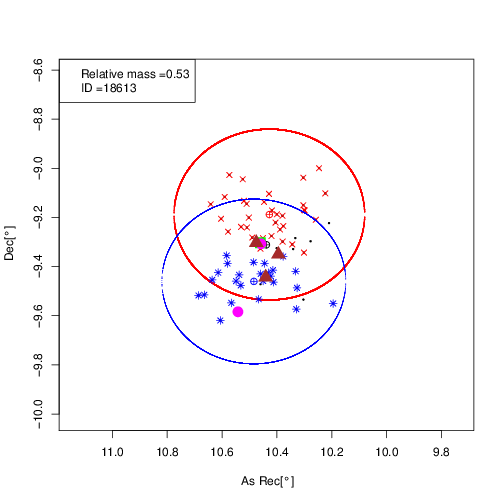
\includegraphics[scale=0.25]{./18613.png}
  \end{figure}
 \end{column}
 \begin{column}{2cm}
 Abell 2029/2033
  \begin{figure}  
   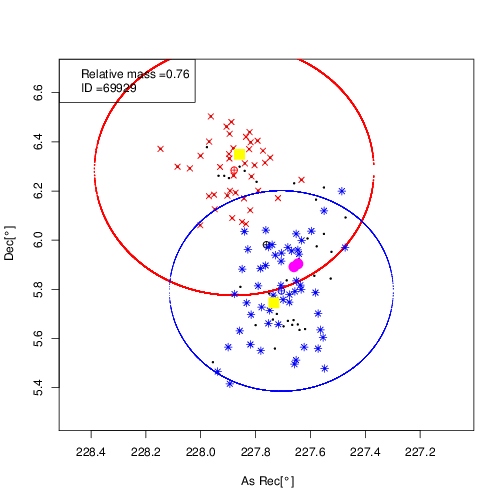
\includegraphics[scale=0.25]{./69929.png}
 % 18613.pdf: 504x504 pixel, 72dpi, 17.78x17.78 cm, bb=0 0 504 504
  \end{figure}
 \end{column}
\end{columns}
 
}

\frame{\frametitle{The non gravitational interactions of dark matter in galaxy clusters. \textit{Harvey et al. 2015}}

\begin{figure}[h!]
 \centering
 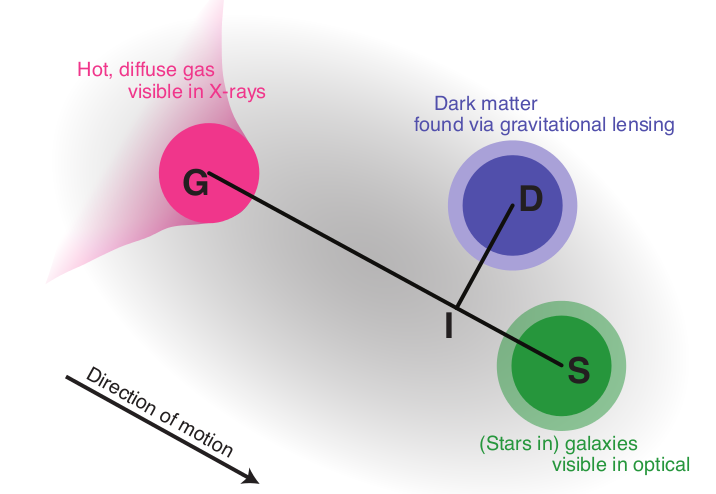
\includegraphics[scale=0.2]{./massey1.png}
  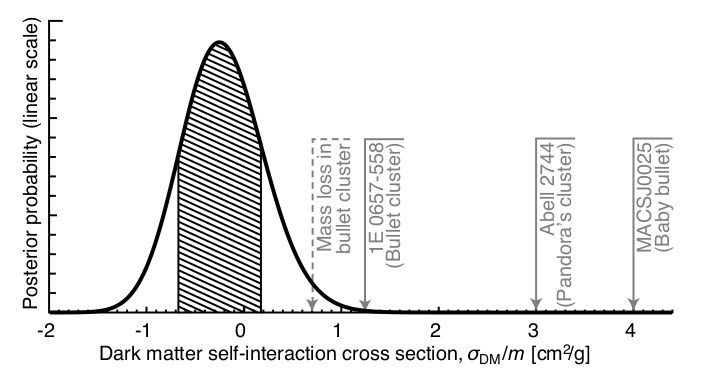
\includegraphics[scale=0.2]{./massey4.png}
 % massey1.png: 716x494 pixel, 72dpi, 25.26x17.43 cm, bb=0 0 716 494
\end{figure}

$\sigma_{DM}/m \leq 0.47$ $cm^{2}/g$ ($95 \% CL$)

}

%\frame{
%\begin{columns}
% \begin{column}{2cm}
% Abell 1424
%  \begin{figure}[h!]
%   \centering
%   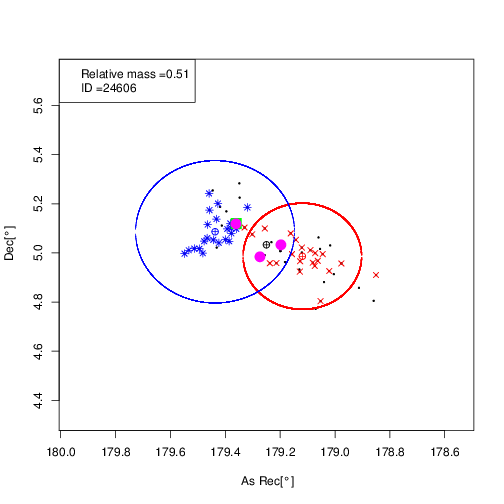
\includegraphics[scale=0.25]{./24606.png}
%  \end{figure}
% \end{column}
% \begin{column}{2cm}
% Abell 1913
%  \begin{figure}
%   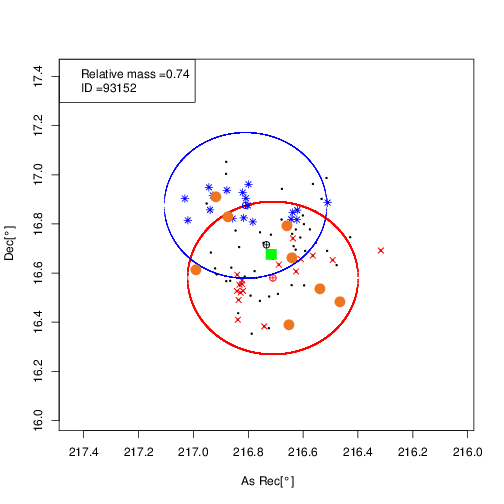
\includegraphics[scale=0.25]{./93152.png}
 % 18613.pdf: 504x504 pixel, 72dpi, 17.78x17.78 cm, bb=0 0 504 504
%  \end{figure}
% \end{column}
%\end{columns}

%}
%------------------------------------------------------------------------------------------------------------------------------------------------
%------------------------------------------------------------------------------------------------------------------------------------------------
%------------------------------------------------------------------------------------------------------------------------------------------------
%------------------------------------------------------------------------------------------------------------------------------------------------
%------------------------------------------------------------------------------------------------------------------------------------------------
%------------------------------------------------------------------------------------------------------------------------------------------------
%------------------------------------------------------------------------------------------------------------------------------------------------

\section{Future work.}
\frame{
\tableofcontents[ 
    currentsection, 
    hideothersections, 
    sectionstyle=show/hide, 
    sectionstyle=show/shaded, 
    ] 
}

\frame{\frametitle{Future work.}
\begin{itemize}
\item Apply the detection method to more deep real catalogs. \pause
 \item Study the physics properties of the galaxies that belong to the identified substructures. \pause
\item Perform astrophysical test over our sample of colliding cluster candidates of the catalog looking for
impose some constraints on dark matter particle properties. \pause
\item Construct a catalog of relaxed clusters in order to study the dark matter equation of state. \pause
\item Reconstruct the 3d merger with the Bayesian techniques presented by \textit{Dawson et al. 2012}.
\end{itemize}


}

\begin{frame}[plain]
\begin{figure}[h!]
 \centering
 
\includegraphics[scale=0.4]{./gracias.png}
 % gracias.png: 657x518 pixel, 72dpi, 23.18x18.27 cm, bb=0 0 657 518
\end{figure}
\end{frame}
\end{document}

